% Preamble
\documentclass[xcolor=dvipsnames]{beamer}
\usetheme{madrid}

% Packages
\usepackage[english,ngerman]{babel}
\usepackage[utf8]{inputenc}
\usepackage{amsmath}
\usepackage{graphicx}
\usepackage{ifthen} % Boolean variables
\usepackage{subfigure} % Horizontal pictures

\definecolor{hBlue}{RGB}{55,118,165}
\usecolortheme[named=hBlue]{structure}

% Distiction between work and stream presentation
\newboolean{work}
\setboolean{work}{false}

\ifthenelse{\boolean{work}}{
    \titlegraphic{
\includegraphics[width=4cm]{../images/logo.png}}
}{}
\title{Gesundheit \& Ernährung}
\subtitle{Makronährstoffe: Kohlenhydrate}
\ifthenelse{\boolean{work}}{
    \author{Adrian Helberg}
    \date{16.06.2021}
}{
    \subtitle{twitch.tv/bl1nzlar}
    \author{Bl1nzlar}
    \date{\today}
}


% Document
\begin{document}

    \maketitle

    \frame{\frametitle{Agenda}\tableofcontents}

    \section{Theorie}
    {
    \setbeamercolor{normal text}{fg=hBlue}\usebeamercolor*{normal text}
    \begin{frame}
        \begin{center}
            \Huge Theorie
        \end{center}
    \end{frame}
    }

    \subsection{Profil}
    \begin{frame}
        \frametitle{Profil}

        \begin{block}{Was sind Kohlenhydrate?}
            \begin{itemize}
                \setlength\itemsep{1em}
                \item Grundbaustein der Pflanzen
                \item Kohlenstoffdioxid + Wasser + Sonne (Photosynthese)
                \item Das Kohlenhydrat, dass bei der Photosynthese herauskommt ist der Traubenzucker, als fester, energiereicher Stoff
                \item Unentbehrlich für das Leben auf der Erde
            \end{itemize}
        \end{block}

        \begin{figure}
            \centering
            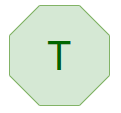
\includegraphics[width=1cm]{../images/t.png}
            \caption{Kohlenhydrat Traubenzucker}
        \end{figure}
    \end{frame}

    \subsection{Traubenzucker}
    \begin{frame}[allowframebreaks]
        \frametitle{Einfachzucker: Traubenzucker}

        \begin{block}{Traubenzucker}
            \begin{itemize}
                \setlength\itemsep{1em}
                \item Alle Lebewesen haben sich um den Traubenzucker als Energiequelle entwickelt
                \item Jede Zelle unseres Körpers kann Traubenzucker zu Energie verbrennen
                \item Traubenzucker lässt sich zu Ketten verbinden
            \end{itemize}
        \end{block}

        \begin{figure}
            \centering
            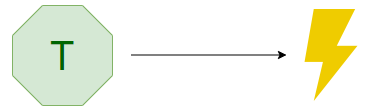
\includegraphics[width=3cm]{../images/t_energie.png}
        \end{figure}

        \framebreak

        \begin{figure}
            \centering
            \subfigure[]{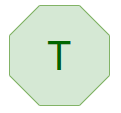
\includegraphics[width=1cm]{../images/t.png}}
            \subfigure[]{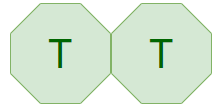
\includegraphics[width=2cm]{../images/t_2.png}}
            \subfigure[]{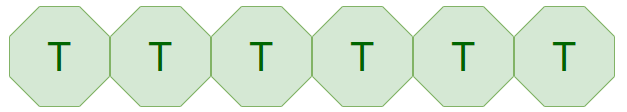
\includegraphics[width=5.4cm]{../images/t_n.png}}
            \caption{(a) Einfachzucker (b) Zweifachzucker (c) Mehrfachzucker}
        \end{figure}

        \framebreak

        \begin{figure}
            \centering
            \subfigure[]{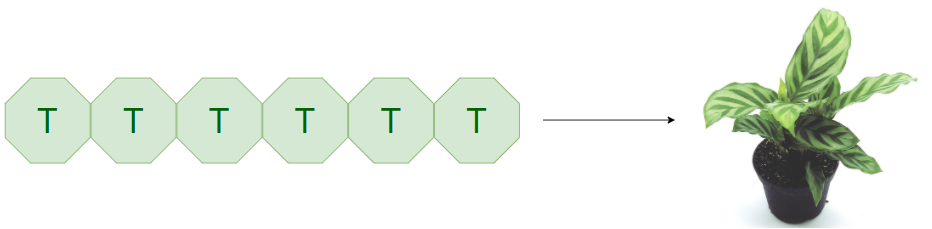
\includegraphics[width=8cm]{../images/pflanzenfasern.png}}
            \subfigure[]{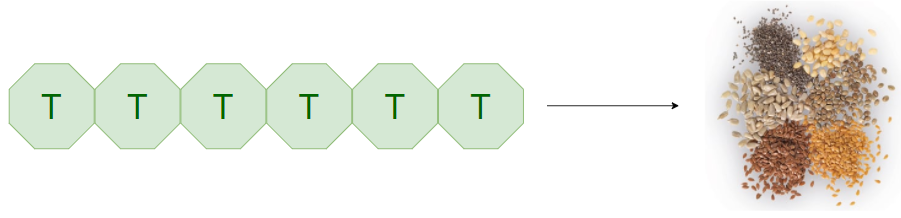
\includegraphics[width=8cm]{../images/samen.png}}
            \caption{(a) Mehrfachzuckerketten als Cellulose ist schwer wieder aufzuspalten und somit schwer verdaulich
                     (b) Pflanzen speichern ihren Mehrfachzucker, der schnell aufgespalten werden soll, zB. in Samen als \textbf{Stärke}}
        \end{figure}

        \framebreak

        \begin{block}{Getreidesamen}
            \begin{itemize}
                \item Weizen, Roggen
                \item Hafer
                \item Reis
                \item Mais
            \end{itemize}
        \end{block}

        \begin{block}{Hülsenfrüchte}
            \begin{itemize}
                \item Bohnen
                \item Linsen
                \item Erbsen
            \end{itemize}
        \end{block}

        \begin{block}{Wurzeln und Knollen}
            \begin{itemize}
                \item Kartoffeln
            \end{itemize}
        \end{block}
    \end{frame}

    \subsection{Fruchtzucker}
    \begin{frame}[allowframebreaks]
        \frametitle{Einfachzucker: Fruchtzucker}

        \begin{block}{Fruchtzucker}
            \begin{itemize}
                \setlength\itemsep{1em}
                \item Kommt in der Natur eher selten vor
                \begin{itemize}
                    \item Reifes Obst
                    \item Bienenhonig
                \end{itemize}
                \item Süßer als Traubenzucker
                \item Fester Bestandteil von Kristallzucker (50\%)
            \end{itemize}
        \end{block}

        \begin{figure}
            \centering
            \subfigure[]{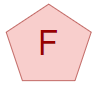
\includegraphics[width=1cm]{../images/F.png}}
            \subfigure[]{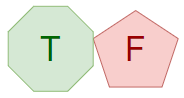
\includegraphics[width=1.8cm]{../images/zucker.png}}
            \caption{(a) Kohlenhydrat Fruchtzucker (b) Haushaltszucker}
        \end{figure}

        \framebreak

        \begin{figure}
            \centering
            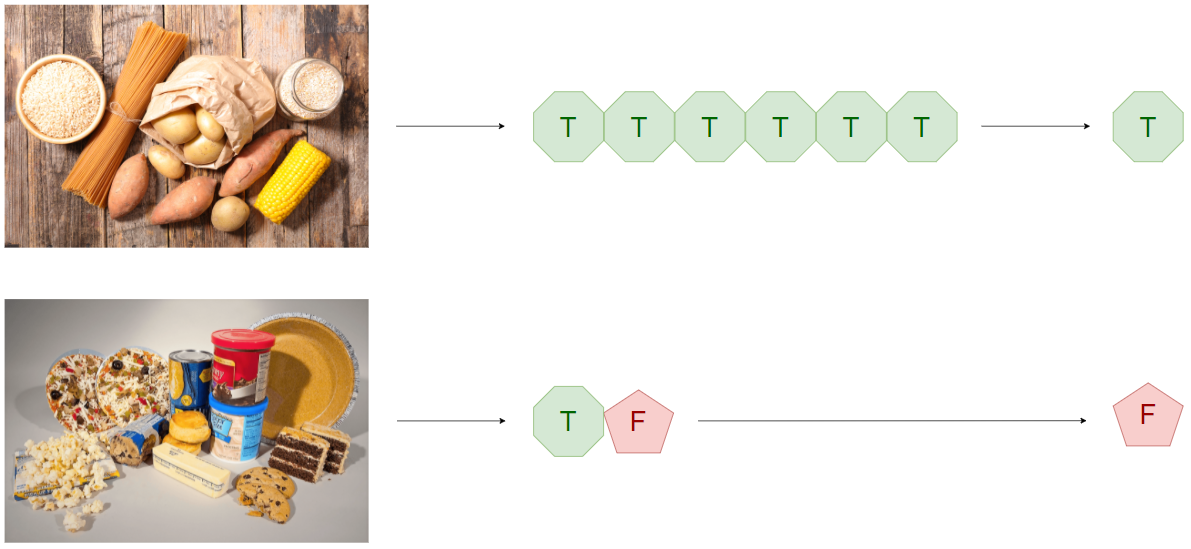
\includegraphics[width=10cm]{../images/t_f.png}
            \caption{Nahrungszucker}
        \end{figure}
    \end{frame}

    \subsection{Stoffwechsel}
    \begin{frame}[allowframebreaks]
        \frametitle{Stoffwechsel}

        \begin{block}{Traubenzucker}
            \begin{itemize}
                \setlength\itemsep{1em}
                \item Kann von jeder Zelle aufgenommen werden
                \item Kann von jeder Zelle zu Energie verbrannt werden
            \end{itemize}
        \end{block}

        \begin{block}{Fruchtzucker}
            \begin{itemize}
                \setlength\itemsep{1em}
                \item Kann \textbf{nur} von der Leber aufgenommen werden
                \item Muss erst in etwas "`brauchbares"' umgewandelt werden
            \end{itemize}
        \end{block}

        \begin{figure}
            \centering
            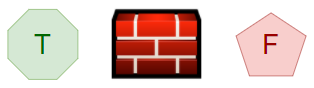
\includegraphics[width=3cm]{../images/wall.png}
            \caption{Traubenzucker und Fruchtzucker sind grundverschieden!}
        \end{figure}

        \framebreak

        \begin{block}{Stärke}
            \begin{itemize}
                \item Makronährstoffe werden im ersten Drittel des Darms aufgenommen
                \item Die Darmwand kann nur Einfachzucker aufnehmen
                \item Aufspaltung in Einfachzucker mithilfe von Verdauungsenzymen
            \end{itemize}
        \end{block}

        \begin{figure}
            \centering
            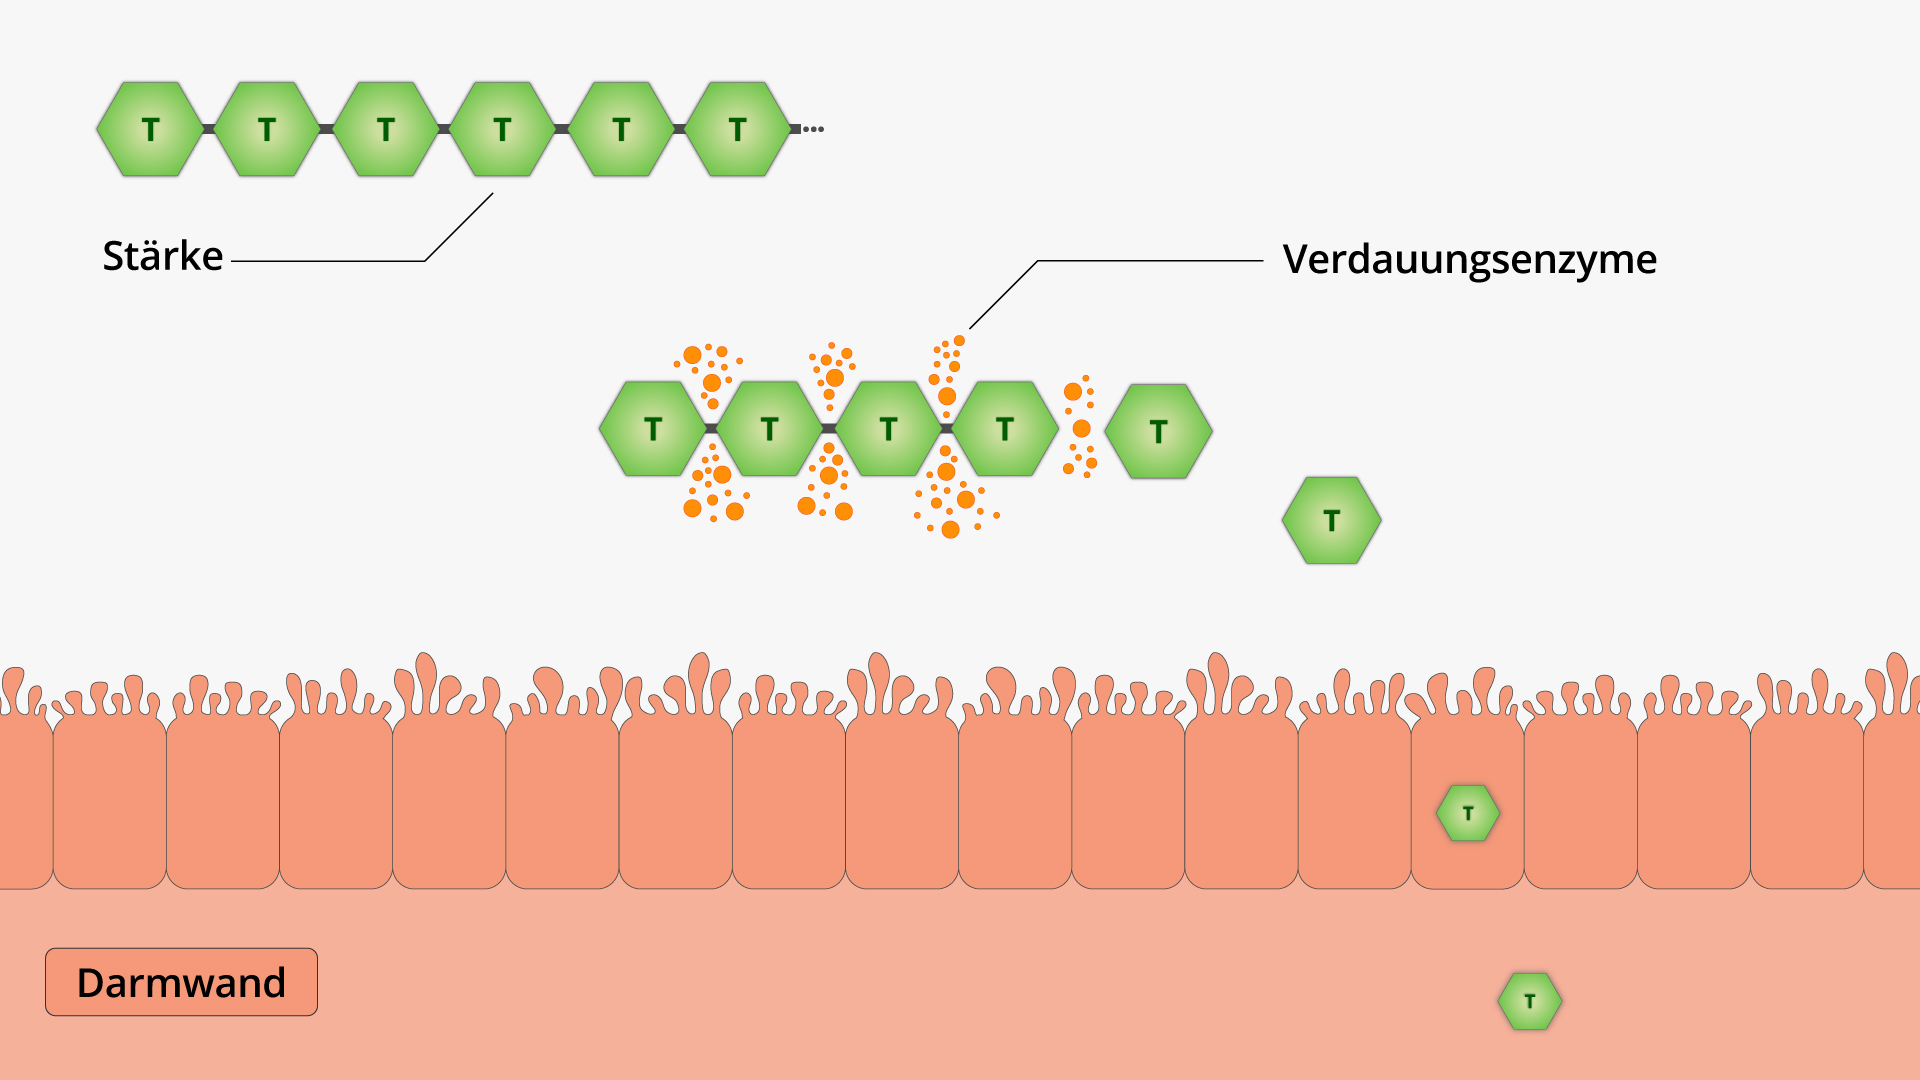
\includegraphics[width=7cm]{../images/verdauung.jpg}
            \caption{Aunahme von Traubenzucker im Dünndarm}
        \end{figure}

        \framebreak

        \begin{figure}
            \centering
            \subfigure[]{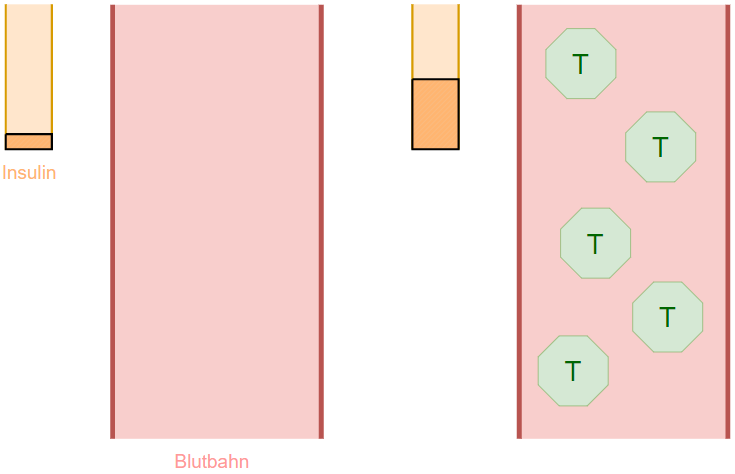
\includegraphics[width=6cm]{../images/blut_1.png}}
            \caption{Anstieg des Blutzuckerspiegels $\rightarrow$ Insulinausschüttung}
        \end{figure}

        \framebreak

        \begin{block}{Insulin}
            \begin{itemize}
                \setlength\itemsep{1em}
                \item Speicher-Hormon
                \item Aufnehmen und Speichern von Nährstoffen (nicht nur Zucker!)
                \item Sorgt nach dem Essen für die Nährstoffaufnahme in Muskeln und Leber
            \end{itemize}
        \end{block}

        \framebreak

        \begin{figure}
            \centering
            \subfigure[]{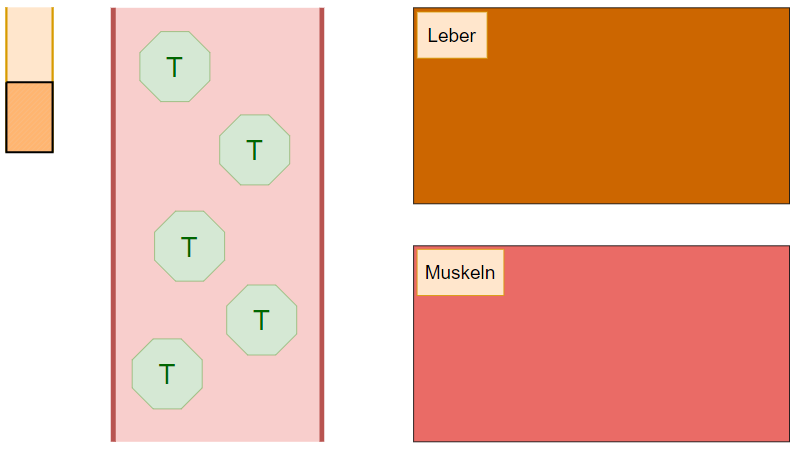
\includegraphics[width=5cm]{../images/blut_2.png}}
            \subfigure[]{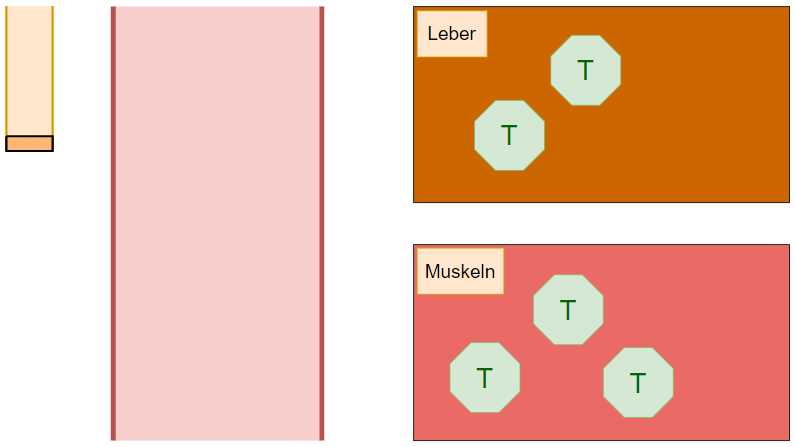
\includegraphics[width=5cm]{../images/blut_3.png}}
            \caption{(a) Hoher und (b) niedriger Blutzuckerspiegel}
        \end{figure}

        \framebreak

        \begin{figure}
            \centering
            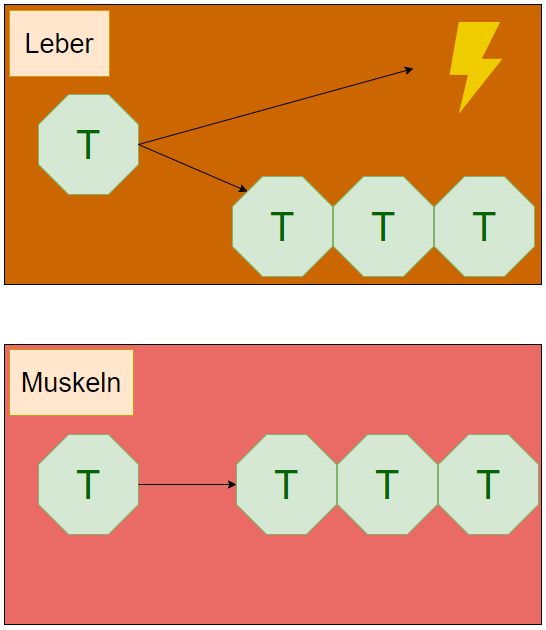
\includegraphics[width=5cm]{../images/leber_1.png}
            \caption{Traubenzucker in Leber und Muskeln}
        \end{figure}

        \framebreak

        \begin{figure}
            \centering
            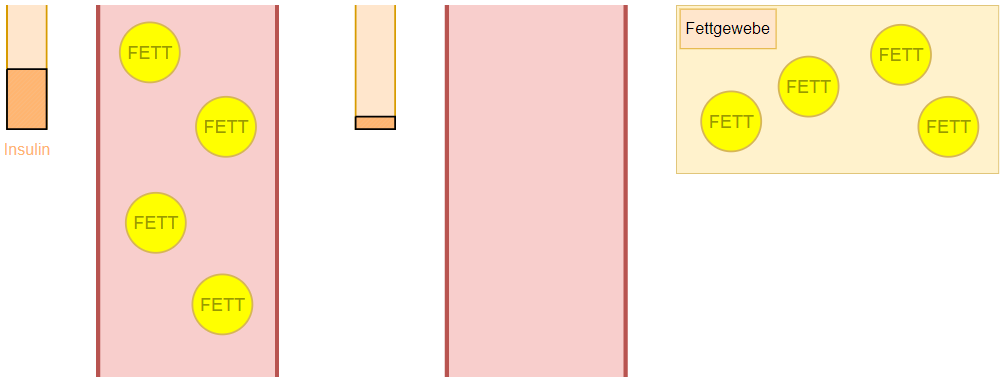
\includegraphics[width=10cm]{../images/fettgewebe.png}
            \caption{Auswirkung Insulin auf Fett}
        \end{figure}

        \framebreak

        \begin{figure}
            \centering
            \subfigure[]{\includegraphics[width=2cm]{../images/nüchtern.png}}
            \subfigure[]{\includegraphics[width=2cm]{../images/nüchtern_1.png}}
            \subfigure[]{\includegraphics[width=2cm]{../images/nüchtern_2.png}}
            \subfigure[]{\includegraphics[width=2cm]{../images/nüchtern_3.png}}
            \caption{(a) Insulinspiegel verdauend (b) Insulinspiegel nüchtern (c) gestörter Insulinspiegel nüchtern (d) gestörter Insulinspiegel verdauend}
        \end{figure}

        \framebreak

        \begin{block}{Gestörter Insulinhaushalt}
            \begin{itemize}
                \setlength\itemsep{1em}
                \item Bei chronisch hohem Insulinspiegel, ist der Fettstoffwechsel zugunsten des Fettaufbaus und entgegen des Fettabbaus verlagert
                \item Ist neben entzündeten Fettzellen die treibende Kraft bei Gewichtszunahme und Übergewicht
                \item Wie kommt es nun zu einem chronisch hohen Insulinspiegel?\\ $\rightarrow$ Stichwort Insulinresistenz
            \end{itemize}
        \end{block}
    \end{frame}

    \subsection{Insulinresistenz}
    \begin{frame}[allowframebreaks]
        \frametitle{Insulinresistenz}

        \begin{figure}
            \centering
            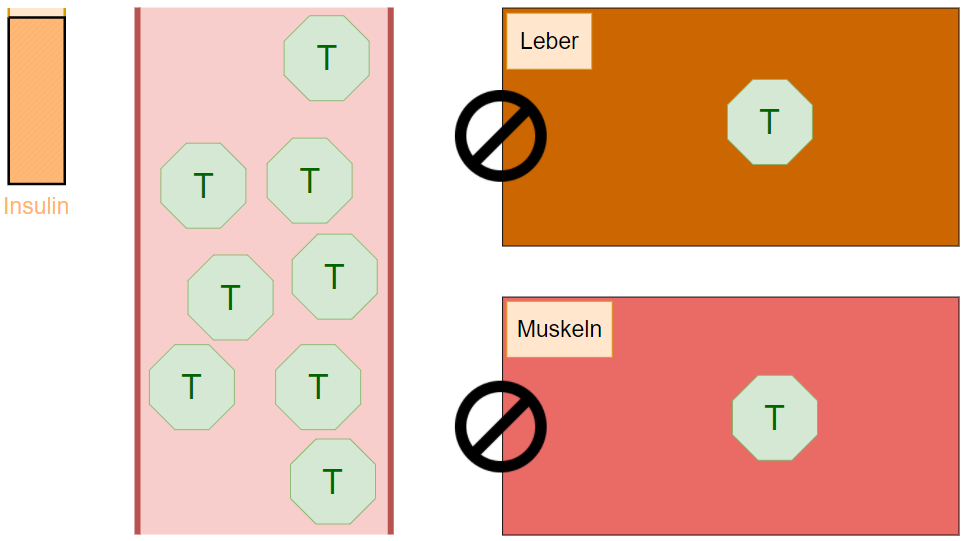
\includegraphics[width=10cm]{../images/resistenz.png}
            \caption{Gestörte Insulinempfindlichkeit der Zellen}
        \end{figure}

        \framebreak

        \begin{block}{Problem 1: Bauspeicheldrüse}
            \begin{itemize}
                \setlength\itemsep{1em}
                \item Bei jeder Nahrungsaufnahme ist der Insulinspiegel extrem hoch
                \item Erschöpfungssyndrom der Bauchspeicheldrüse durch Überproduktion von Insulin $\rightarrow$ Diabetes Typ II
                \item Nicht nur Fett, sondern alle Nährstoffe werden vermindert in das Blut zurückgegeben (Fettstoff\textbf{wechsel})
                \item Bauchfett ist besonders Insulinresistenz und stoffwechselaktiv
            \end{itemize}
        \end{block}

        \framebreak

        \begin{block}{Problem 2: Leber}
            \begin{itemize}
                \item Ein hoher Insulinspiegel veranlasst die Leber viel Traubenzucker in Fett umzuwandeln, das ins Blut abgegeben wird (die Leber "reinigt sich" vom Traubenzucker)
                \item Zum erhöhten Blutzucker kommt nun auch erhöhtes Blutfett
            \end{itemize}
        \end{block}

        \begin{figure}
            \centering
            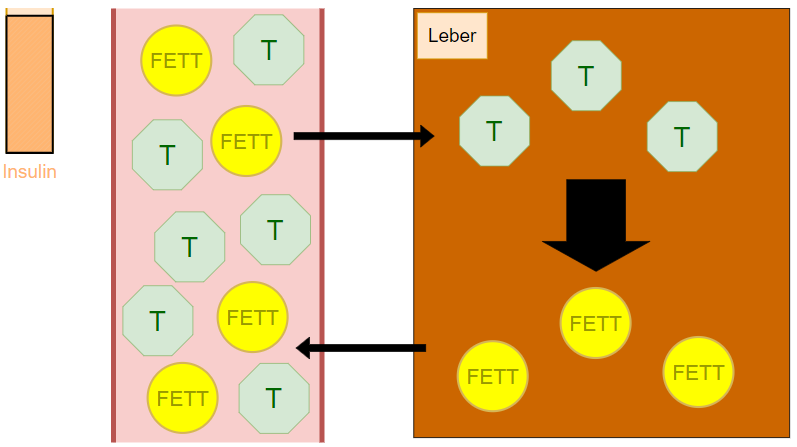
\includegraphics[width=6cm]{../images/problem_leber.png}
            \caption{Hohe Blutfette durch Insulinresistenz}
        \end{figure}

        \framebreak

        \begin{block}{Problem 3: Cholesterin}
            \begin{itemize}
                \setlength\itemsep{1em}
                \item $\rightarrow$ Vortrag 30.06. Makronährstoffe: Fett
            \end{itemize}
        \end{block}

        \framebreak

        \begin{block}{Problem 4: Blutdruck}
            \begin{itemize}
                \setlength\itemsep{1em}
                \item Ein hoher Insulinspiegel führt zu Bluthochdruck
                \item Die Nieren scheiden weniger Natrium aus (Insulin hoch $\rightarrow$ Nährstoffe \textbf{aufnehmen}, Insulin niedrig $\rightarrow$ Nährstoffe abgeben)
                \item Natrium erhöht den Blutdruck
            \end{itemize}
        \end{block}

        \framebreak

        \begin{figure}
            \centering
            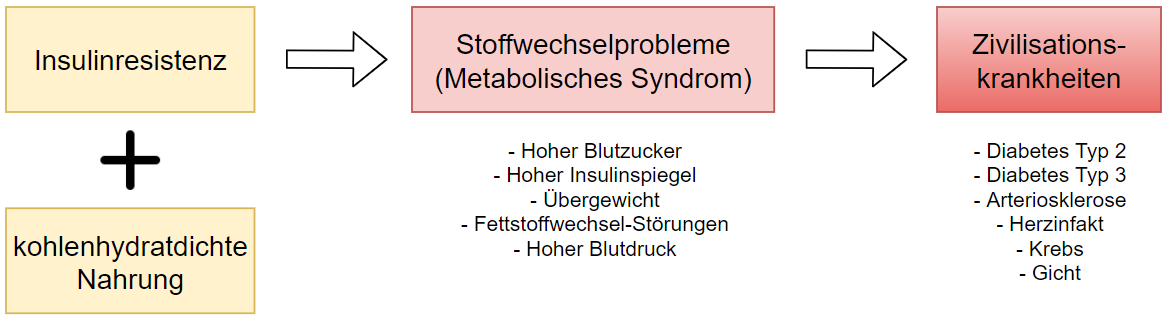
\includegraphics[width=12cm]{../images/problem_zusammenfassung.png}
            \caption{Zusammenfassung: $\rightarrow$ Was sind die Ursachen für Insulinresistenz?}
        \end{figure}

        \framebreak

        \begin{block}{Ursache 1: Stress}
            \begin{itemize}
                \item In Stresssituationen soll der Blutzucker hoch sein, damit die Energie (Traubenzucker) für die Zellen schneller verfügbar ist
                \item Nerven und Muskeln sind nicht auf das Insulin zur Aufnahme von Traubenzucker angewiesen
                \item Dauerhafter Stress macht die Zellen dauerhaft Insulinresistent
            \end{itemize}
        \end{block}

        \begin{figure}
            \centering
            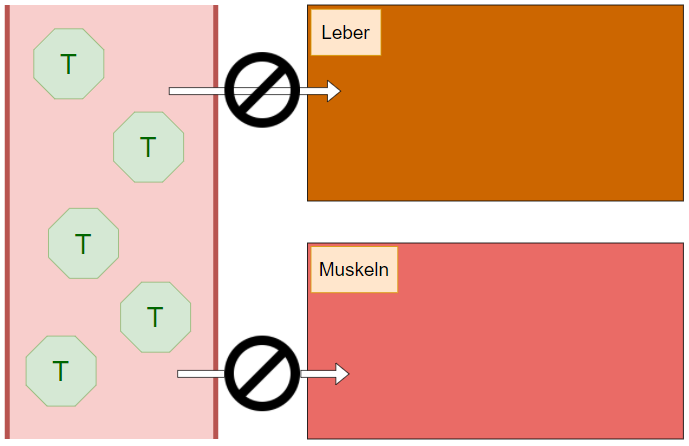
\includegraphics[width=4cm]{../images/ursache_1.png}
            \caption{Stressbedingte Insulinresistenz}
        \end{figure}

        \framebreak

        \begin{block}{Ursache 2: Überernährung}
            \begin{itemize}
                \item Glykogenspeicher der Muskeln sind voll (durschnittlich 500g)
                \item Zellen schützen sich vor freiem Traubenzucker mit Insulinresistenz
            \end{itemize}
        \end{block}

        \begin{figure}
            \centering
            \subfigure[]{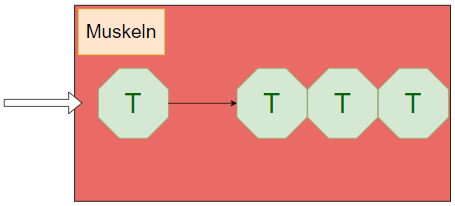
\includegraphics[width=4cm]{../images/ursache_2.png}}
            \subfigure[]{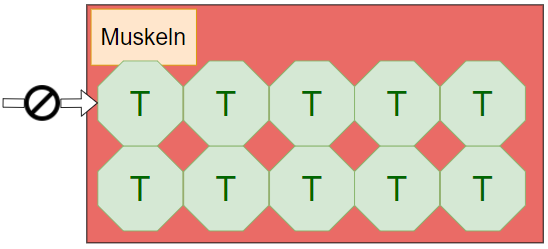
\includegraphics[width=4cm]{../images/ursache_2_2.png}}
            \caption{(a) normale Aufnahme (b) volle Glykogenspeicher
            }
        \end{figure}

        \framebreak

        \begin{block}{Ursache 3: Bewegungsmangel}
            \begin{itemize}
                \setlength\itemsep{1em}
                \item Untersuchung am "`Copenhagen Muscle Research Center"', 2011
                \item 12 jungle und gesunde Männer
                \item 7 Tage totale Bettruhe
                \item Gesteigerte Insulinresiszenz als Effekt auf die Muskeln
            \end{itemize}
        \end{block}

        \framebreak

        \begin{block}{Ursache 4: Fettleber}
            \begin{itemize}
                \item Alkohol wird zu Fett, das sich in der Leber konzentriert abgebaut
                \item Überangebot von Traubenzucker
                \item Fruchtzucker (!)
            \end{itemize}
        \end{block}

        \begin{figure}
            \centering
            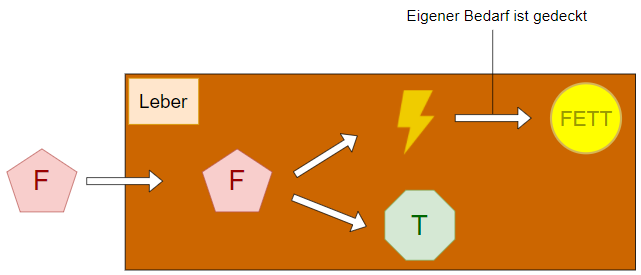
\includegraphics[width=8cm]{../images/ursache_3.png}
            \caption{Leberverfettung durch Überangebot an Fruchtzucker}
        \end{figure}
    \end{frame}

    \subsection{Fruchtzuckerkonsum}
    \begin{frame}{Fruchtzuckerkonsum}
        \begin{block}{1850}
            \begin{itemize}
                \setlength\itemsep{1em}
                \item 4g Fruchtzucker am Tag
                \item Einzige Quelle: Obst
            \end{itemize}
        \end{block}

        \begin{block}{Heute}
            \begin{itemize}
                \setlength\itemsep{1em}
                \item $>$50g Fruchtzucker am Tag
                \item Quelle: Kristallzucker (50\% Traubenzucker 50\% Fruchtzucker)
            \end{itemize}
        \end{block}

        \begin{block}{Späterer Vortrag}
            \begin{itemize}
                \setlength\itemsep{1em}
                \item Insulinresistenz und Leptinunterdrückung\\ $\rightarrow$ Schlüssel zum langfristigen Schlanksein
            \end{itemize}
        \end{block}
    \end{frame}

    \section{Praxis}
    {
        \setbeamercolor{normal text}{fg=hBlue}\usebeamercolor*{normal text}
        \begin{frame}
            \begin{center}
                \Huge Praxis
            \end{center}
        \end{frame}
    }

    \begin{frame}{Tipps \& Tricks}
        \begin{itemize}
            \setlength\itemsep{1em}
            \item Hochkonzentrierte Fruktose vermeiden
            \begin{itemize}
                \item Gezuckerte Getränke
                \item Fruchtsäfte
            \end{itemize}
            \item Etiketten lesen
            \begin{itemize}
                \item Versteckten Zucker erkennen:\\ Dextrin, Dextrose, Dicksaft, Fruchtextrakt, Fruchtsaftkonzentrat, Fructose-Glucose-Sirup, Gerstenmalz(extrakt), Matose
                \item Achsamkeit entwickeln
            \end{itemize}
            \item Lebensmittel statt Nahrungsmittel
        \end{itemize}
    \end{frame}

    \section{Fragerunde}
    {
        \setbeamercolor{normal text}{fg=hBlue}\usebeamercolor*{normal text}
        \begin{frame}
            \begin{center}
                \Huge Fragerunde
            \end{center}
        \end{frame}
    }

\end{document}